\documentclass[12pt]{beamer}
\usetheme{Malmoe}
\usepackage{siunitx}
\usepackage{hyperref}
\usepackage{cancel}
\sisetup{
  per-mode = fraction,
  fraction-function = \frac
}
\usepackage{extpfeil} %for the arrows

\usepackage{tikz}
\usepackage{graphicx}  % To include images
\usetikzlibrary{shapes.geometric, arrows}

% Define block styles for the flowchart
\tikzstyle{process} = [rectangle, minimum width=2.4cm, minimum height=0.5cm, text centered, draw=black, fill=blue!10]
\tikzstyle{imageblock} = [rectangle, minimum width=2.4cm, minimum height=1.5cm, text centered] % New style for image node
\tikzstyle{arrow} = [thick,->,>=stealth]

\begin{document}


\title{Paper Presentation: Depth Anything}
\subtitle{\begin{itemize}
        \item Depth Anything: Unleashing the Power of Large-Scale Unlabeled Data (V1)
        \item Depth Anything V2 (V2)
    \end{itemize}}
\author{Benjamin Stadler}
\institute{Tsinghua University \\
    Machine Vision (Fall 2024) \\
Contact: \texttt{\href{mailto:bestadle@ethz.ch}{bestadle@ethz.ch}}}
\date{October 2024}


\begin{frame}
\titlepage
\end{frame}


\begin{frame}
    \frametitle{At a Glance}

    \begin{itemize}
        \item[What] Molecular Depth Estimation (MDE)
        \item[Who] HKU, TikTok
        \item[When] April 2024 (V1), June 2024 (V2)
        \item[How]
        \begin{itemize}
            \item[V1] known techniques + train with \underline{unlabeled data}
            \item[V2] technique from V1 + train with \underline{synthetic data}
        \end{itemize}
    \end{itemize}
    
    \begin{figure}
        \centering
        \includegraphics[width=0.49\textwidth]{./figures/huashan_orig.jpg}
        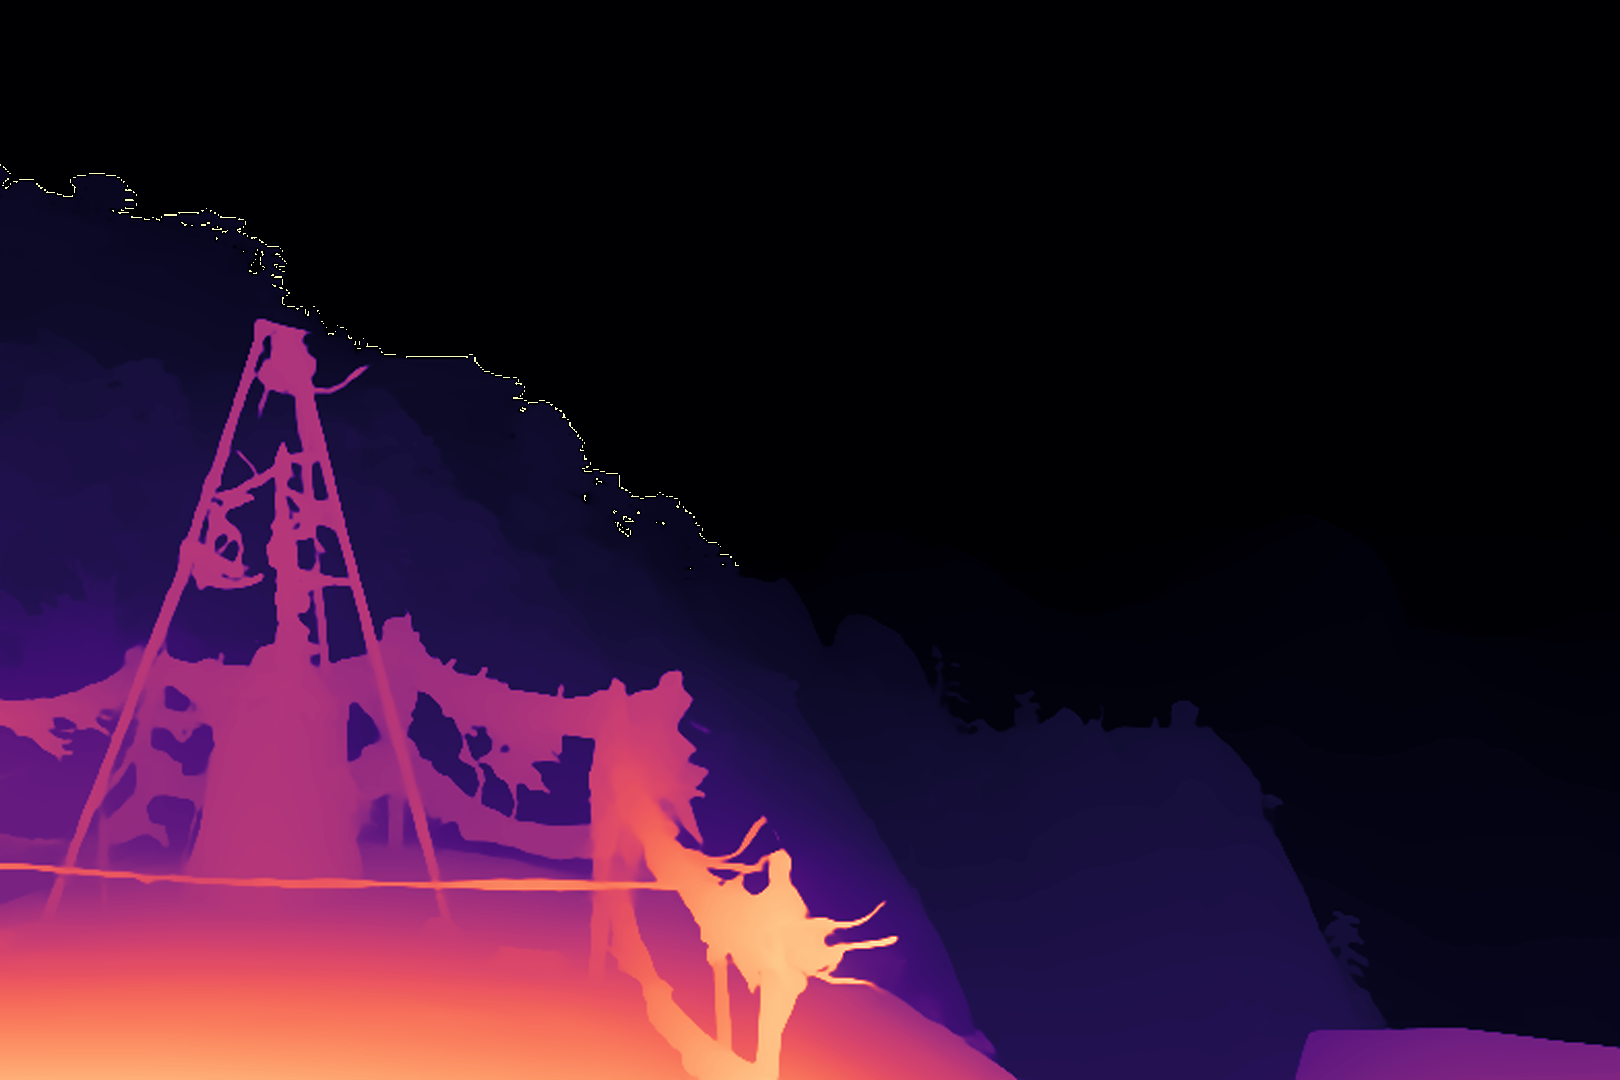
\includegraphics[width=0.49\textwidth]{./figures/huashan_depthmap.png}
        \caption{Sample Input $\to$ Output (V2, large model)}
        \label{fig:intro}
    \end{figure}

\end{frame}

%have a teacher, student model; with segmentation
\begin{frame}
    \frametitle{Architecture V1}
    \framesubtitle{Overview}
    
    \begin{columns}
        
        \column{0.4\textwidth}
        
        \textbf{Datasets}
        \begin{equation*}
            \begin{aligned}
                \underbrace{\mathcal{D}^l}_{\text{labeled}} &= 
                \begin{cases} 
                    \text{6 Datasets} \\ 
                    \text{1.5M Images} 
                \end{cases} \\
                \underbrace{\mathcal{D}^u}_{\text{unlabeled}} &= 
                \begin{cases} 
                    \text{8 Datasets} \\ 
                    \text{62M Images} 
                \end{cases}
            \end{aligned}
        \end{equation*}
        \pause
        \begin{itemize}
            \item[Key] MiDaS $\leadsto$ Loss Function\footnote{Mixing Datasets for
            Zero-shot Cross-dataset Transfer}
        \end{itemize}
        
        
        \column{0.6\textwidth}
        \pause
        \textbf{Training Process}
        \begin{enumerate}
            \item<4-> Training Teacher $T$ with $\mathcal{D}^l$
            
            \item<5-> Use $T$ to \underline{pseudo-label}:
            \\$\mathcal{D}^u \xlongrightarrow{T} \hat{\mathcal{D}}^u $
            
            \item<6-> Training Student $S$ with $\hat{\mathcal{D}}^u \cup \mathcal{D}^l$
        \end{enumerate}
    
    \end{columns}
\end{frame}



\begin{frame}
    \frametitle{Architecture V1}
    \framesubtitle{Details}
    
    \begin{columns}
        \column{0.4\textwidth}
        \begin{tikzpicture}[node distance=2cm]
            
            % Nodes
             \node (startImage) [imageblock] {\includegraphics[width=2cm]{./figures/tianjin_orig.JPG}};
            \node (perturbations) [process, below of=startImage, yshift=0.8cm] {\small Perturbations};
            \node (imageMiddle) [imageblock, below of=perturbations, yshift=+0.8cm] {
\includegraphics[width=2cm]{./figures/cutmix_example.png}};
            \node (encoderStatic) [process, below of=imageMiddle, yshift=0.8cm, xshift=-1.3cm] {\small Encoder Static};
            \node (encoderDynamic) [process, below of=imageMiddle, yshift=0.8cm, xshift=1.3cm] {\small Encoder};
            \node (decoder) [process, below of=encoderStatic, yshift=1.2cm, xshift=1.3cm] {\small Decoder};
            \node (imageEnd) [imageblock, below of=decoder, yshift=+0.8cm] {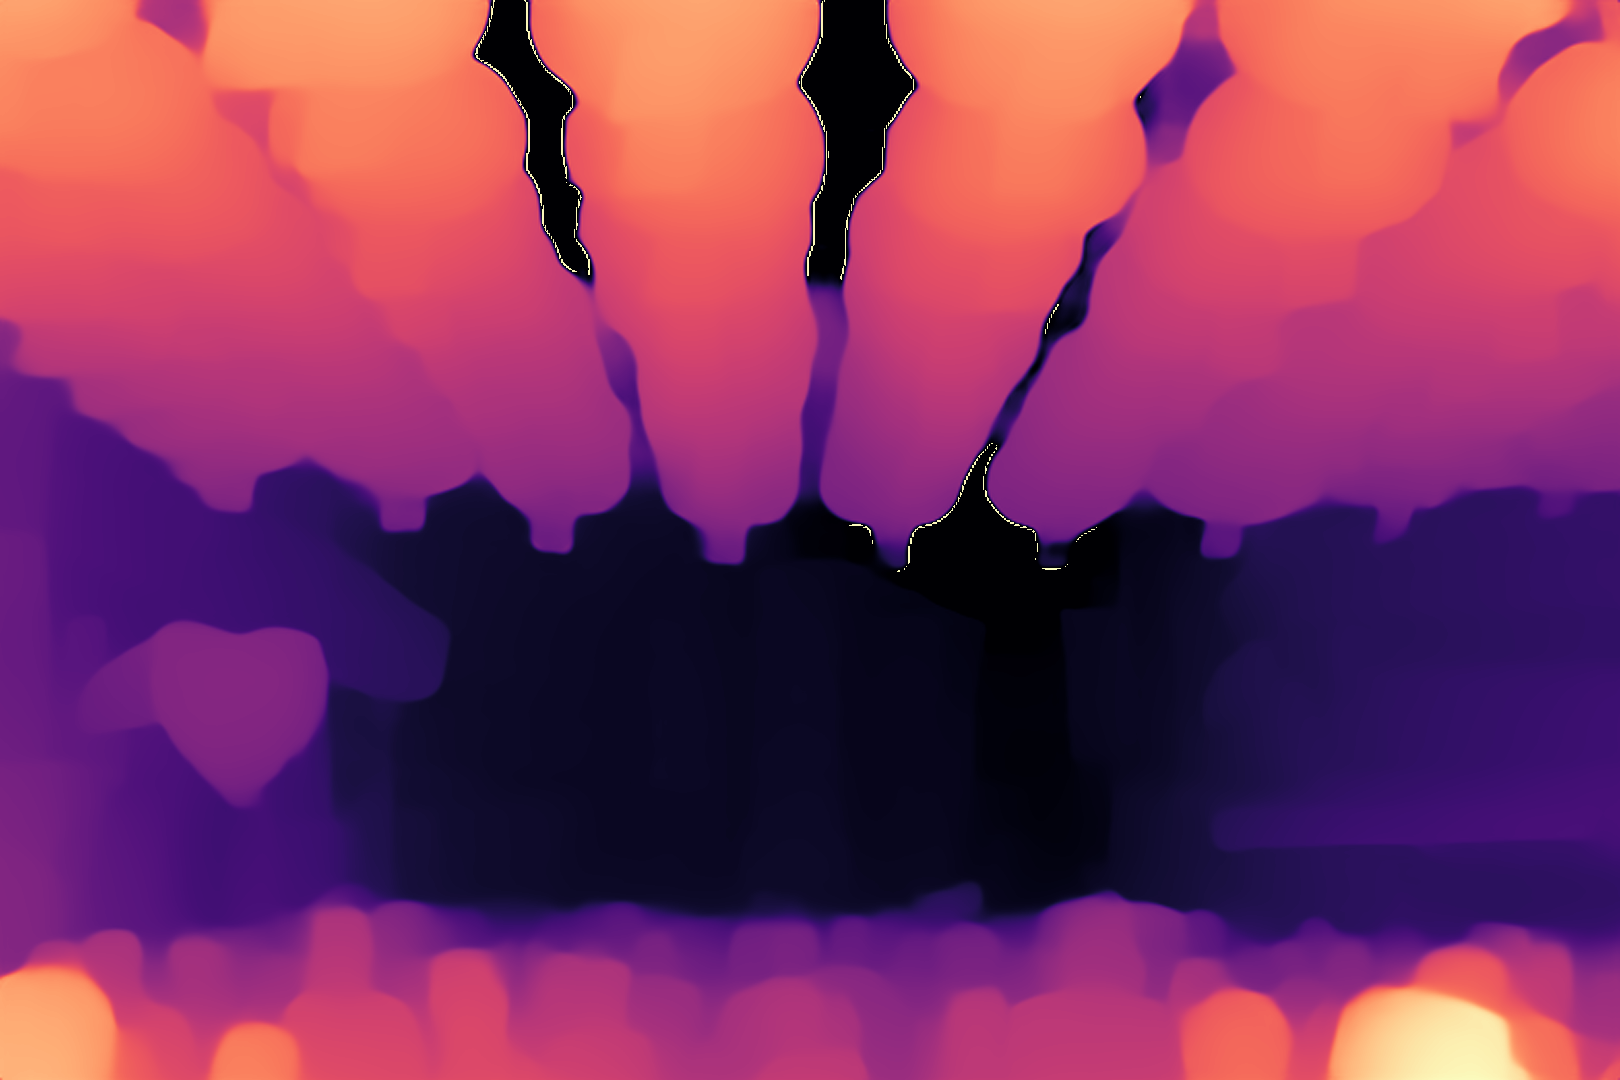
\includegraphics[width=2cm]{./figures/tianjin_depthmap_v1-small.png}};
            
            % Arrows
            \draw [arrow] (startImage) -- (perturbations);
            \draw [arrow] (perturbations) -- (imageMiddle);
            \draw [arrow] (imageMiddle) -- (encoderStatic);
            \draw [arrow] (imageMiddle) -- (encoderDynamic);
            \draw [arrow] (encoderDynamic) -- (decoder);
            \draw [arrow] (encoderStatic) -- (decoder);
            \draw [arrow] (decoder) -- (imageEnd);
            
        \end{tikzpicture}
    
        \column{0.6\textwidth}
        \pause
        
        \begin{itemize}
            \item<2-> Perturbations (only for $S$)
            \begin{itemize}
                \item[$\in\hat{\mathcal{D}}^u$] color shift + CutMix
                \item[$\in\mathcal{D}^l$] horizontal flip
            \end{itemize}
            $\leadsto$ be more robust
        
            \item<3-> Encoders
            \begin{itemize}
                \item[Normal] $\leftarrow$ DINOv2 encoder
                \item[Static] $\leftarrow$ frozen DINOv2 encoder
                \item Linked by a feature alignment loss
            \end{itemize}
            $\leadsto$ auxiliary supervision
            
            \item<4-> Decoder $\leftarrow$ DPT decoder (as in MiDaS)
            
        \end{itemize}
    \end{columns}
    
\end{frame}

\begin{frame}
    \frametitle{Architecture V2}
\end{frame}


%quantative and qualitative results; note that fine details hard to compare
\begin{frame}
    \frametitle{Results}
\end{frame}

\begin{frame}
    \frametitle{Live Demo}
    
\end{frame}

% graphical overview
\begin{frame}
    \frametitle{Summary}
\end{frame}


\begin{frame}
    \frametitle{Sources}
    \tiny
    
    \textbf{Presentation \& Code} \href{https://github.com/birawaich/thu_mavi_paperpresentation}{Github}
    
    \textbf{Papers}
    \begin{itemize}
        \item \href{https://arxiv.org/abs/2401.10891}{Depth Anything: Unleashing the Power of Large-Scale Unlabeled Data}
        \item \href{https://arxiv.org/abs/2406.09414}{Depth Anything V2}
        \item \href{https://arxiv.org/abs/1907.01341}{MiDaS}
        \item \href{https://arxiv.org/abs/2304.07193}{DINOv2}
        \item \href{https://arxiv.org/abs/1905.04899}{CutMix}
    \end{itemize}
    
    \textbf{Pictures}
    if not noted differently, captured myself
    
    \textbf{Illustrations}
    if not noted differently, created myself
    
    
\end{frame}

\end{document}
